\chapter{Analyse en ontwerp}
Uit de probleemstelling werd het snel duidelijk dat het probleem omtrent het Python testraamwerk complexer is dan op het eerste zicht lijkt.
In dit hoofdstuk zal het probleem verder geanalyseerd worden.
Aan de hand van deze bevindingen gaat een architectuur en structuur ontworpen worden.
Deze vormen de basis voor de implementatie van de demo.

\section{Analyse}
Het probleem van Televic was het volgende:
Televic fabriceert producten die moeten voldoen aan strenge veiligheidsnormen.
Om hun producten hierop te kunnen testen heeft Televic een Python testraamwerk ontworpen waarmee het mogelijk wordt om de producten aan verschillende testscenario's te onderwerpen.
Dit testraamwerk maakt gebruik van een grote set aan drivers en bibliotheken om een correcte werking te garanderen.
Een direct gevolg hiervan is dat het installatieproces op een nieuwe testtoren een uitgebreide klus is.
Hiernaast groeit het aantal gebruikers van het testraamwerk continu samen met het aantal drivers en bibliotheken.
Het doel is om een systeem te ontwikkelen dat Televic kan bijstaan bij het installatie en verspreidingsproces.
Een verdere analyse is wel nodig.
Zo is het mogelijk om een applicatie te ontwikkelen die voldoet aan de initiële probleemstelling maar ook uitbreidbaar is naar de toekomst toe.

%Packager
De probleemanalyse onthulde al snel dat dit probleem onder te verdelen is in verschillende deelproblemen.
Het testraamwerk bestaat uit verschillende componenten, hieronder vallen de drivers en bibliotheken.
Elke component heeft een aparte installatiewijze en moeten sommige componenten voor andere geïnstalleerd worden.
Zo zal Python één van de eerste componenten zijn die geïnstalleerd moet worden.
Hiernaast moeten verscheidene componenten geconfigureerd tijdens het installatieproces aan de hand van een configuratiebestand.
Dit configuratiebestand hoort samen met de testtoren waarop het testraamwerk op geïnstalleerd word.
Door gebruik te maken van additionele software worden verschillen in implementaties, door bijvoorbeeld verschillende programmeertalen, opgevangen.
Een stuk van de applicatie zal dus bestaan uit deze additionele software die instaat voor het inpakken van de componenten.
In de rest van de thesis zal naar dit onderdeel de \emph{packager} heten.
Hiervoor kan beroep gedaan worden op verscheidene technologieën, structuren en architecturen die besproken werden in Sectie~\vref{sec:technologieen}.

%Server
De probleemanalyse onthulde ook dat de verschillende executables verspreidt moeten worden.
Door dit proces te automatiseren, is het mogelijk om waardevolle informatie te verzamelen.
Met deze informatie kunnen rapporten gegeneerd worden over het deployment proces.
In Secties~\ref{sec:deployment} - \ref{sec:caseStudies} werden verschillende problemen maar ook oplossingen besproken die aan de basis liggen voor het ontwerp van dit onderdeel van de applicatie. 
In het vervolg van de thesis zal dit onderdeel (dat zal instaan voor het verspreiden van het testraamwerk maar ook voor de communicatie tussen de producten van het testraamwerk en de gebruikers) vermeld worden als de \emph{deployment server}.

%Environment
In Sectie~\vref{sec:softwareLevenscyclus} werd besproken welke problemen kunnen optreden tijdens het installatieproces.
Deze problemen moeten opgevangen worden om een schaalbare oplossing te bedenken voor Televic.
Om dit op te vangen, kan er gebruik gemaakt worden van één (of meerdere) strategieën die besproken werd in Sectie~\vref{sec:rollback}.
Dit onderdeel van de applicatie vooral aanwezig aan de client-side aangezien dat de plaats is waar het testraamwerk aanwezig zal zijn.
In de loop van de thesis zal naar dit onderdeel verwezen worden als de \emph{deployment environment}.

Na de probleemanalyse is het nu duidelijk dat het werk op te delen valt in drie grote componenten.
Deze drie onderdelen zullen de basis vormen voor de architectuur en zullen gebruikt worden als leidraad.
Het eerste onderdeel zal bestaan uit de packager met als doel het inpakken van de nodige drivers, bibliotheken, \ldots .
Naast de packager is er de deployment server instaat voor het verspreiden van de installers die de packager aflevert.
Aan de client-side zal de deployment environment aanwezig zijn waardoor installatie-complicaties vermindert worden door de installatie te isoleren.
Mocht een rollback nodig zijn, dan kan deze op een eenvoudige manier gebeuren.
In Figuur~\vref{fig:overzichtsDiagram} wordt de algemene structuur van de applicatie weergegeven.
Met behulp van deze basis is het mogelijk om een demo te produceren voor de finale verdediging.

\begin{figure}[!hbt]
\centering
  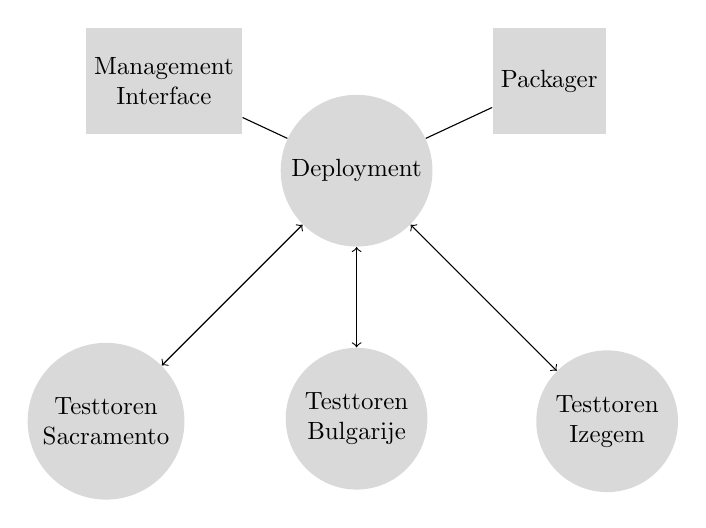
\begin{tikzpicture}[scale=.9, transform shape]
\tikzstyle{every node} = [circle, minimum size = 2cm, fill=gray!30]
\node (a) at (0, 0) {Deployment};
\node[shape = rectangle,minimum size = 1.5cm] (packager) at +(25: 3) {Packager};
\node[shape = rectangle,minimum size = 1.5cm, align=center] (logger) at +(155: 3) {Management\\ Interface};
\node[align=center] (b) at +(225: 5) {Testtoren\\ Sacramento};
\node[align=center] (c) at +(270: 3.5) {Testtoren\\ Bulgarije};
\node[align=center] (d) at +(315: 5) {Testtoren\\ Izegem};
\foreach \from/\to in {a/b, a/c, a/d}
\draw [<->] (\from) -- (\to);
\draw [-] (a) -- (packager);
\draw [-] (a) -- (logger);
\end{tikzpicture}
  \caption{Overzichtsdiagram van de algemene structuur}
  \label{fig:overzichtsDiagram}
\end{figure}

\section{Databank ontwerp}\label{sec:databank}
In de voorgaande Sectie werd aangehaald met welke problemen Televic kampt.
Eén van de problemen is de continue groei van pakketten waar het framework gebruikt van maakt en het aantal gebruikers die het framework gebruiken.
Om dit probleem aan te pakken wordt een databank ontworpen voor het opslaan van alle cruciale data over zowel het installatieproces en alle gebruikers.
In overleg met Televic werd ervoor gekozen om MySQL te gebruiken als managementsysteem.
Het ontwerp van de databank is terug te vinden in Figuur~\vref{fig:databank}.

\begin{figure}[!ht]
\centering
\makebox[0pt]{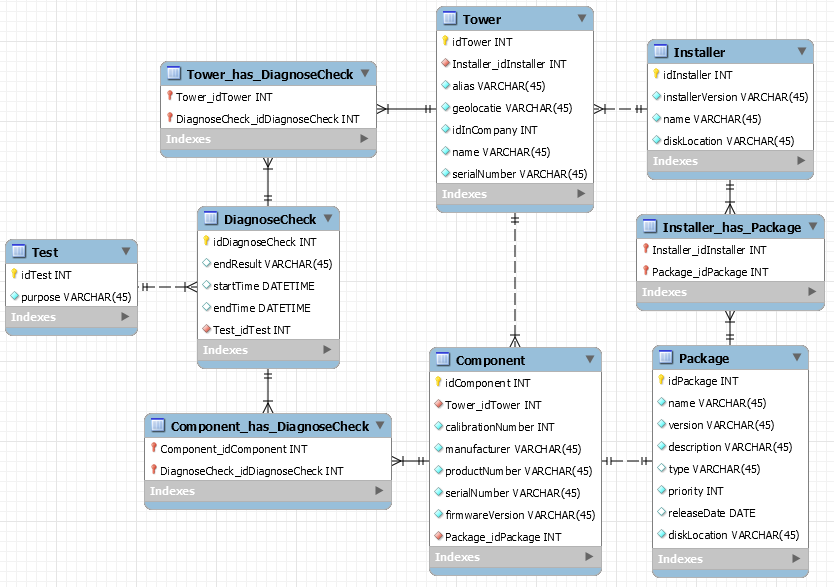
\includegraphics[scale=0.7]{afbeelding/databankOntwerp.png}}
\caption{Ontwerp van de databank}
\label{fig:databank}
\end{figure}

De tabellen tower en hardware\_component dienen om iedere gebruiker, typisch een testtoren of een laptop, te beschrijven.
Iedere toren heeft een ID, naam en serienummer.
De combinatie van deze drie waarden is uniek binnen het bedrijf en de combinatie kan gebruikt worden als identificatie binnen het systeem maar deze combinatie draagt geen betekenis voor een gebruiker.
Om dit op te vangen wordt aan iedere toren een alias gekoppeld waardoor de identificatie voor mensen vlotter kan verlopen.
Elke toren bestaat typisch uit verschillende hardware componenten, zoals voedingen of netwerkkaarten, die nodig zijn om testen uit te voeren.
Iedere component is gemaakt door een bepaalde fabrikant en krijgt van de fabrikant een serienummer.
Vanuit het bedrijf wordt losstaand hiervan een nummer toegekend aan iedere component die gebruikt wordt om de calibratie instellingen te achterhalen.
Iedere hardware component gebruikt firmware om correct te functioneren.
Naast alle bovengenoemde informatie wordt ook de versie van de firmware opgeslagen.
Door het opslaan van al deze informatie wordt het mogelijk om:
\begin{enumerate}
\item Torens van elkaar te onderscheiden
\item Achterhalen welke hardware componenten aanwezig zijn op welke toren
\item Welke firmware versie draait op welke hardware component
\end{enumerate}

Naast informatie over de gebruikers wordt ook informatie over de verschillende installers en pakketten bijgehouden.
Een installer bestaat uit een combinatie van verschillende software pakketten.
Bij deze pakketten moet één pakket aanwezig zijn dat het Python testraamwerk bevat.
Hiernaast zijn verschillende andere pakketten aanwezig voor drivers.
In Figuur~\vref{fig:installerStructuur} is een voorbeeld zichtbaar van een installer die bestaat uit drie verschillende pakketten.
Eén pakket wordt gebruikt door het testraamwerk en de twee anderen voor drivers die nodig zijn om het testraamwerk correct te laten functioneren.
Iedere toren wordt gekoppeld aan één installer en zo aan één testraamwerk.
Hiernaast is het mogelijk om pakketten te koppelen aan hardware componenten.
Zo kan een driver voor een voeding gekoppeld worden aan de entry van de voeding die aanwezig is in de hardware\_component tabel.
Op deze wijze worden de hardware-software afhankelijkheden bijgehouden.
Van ieder pakket wordt bijgehouden welk type pakket het is (een executabel, zip bestand, \ldots), de prioriteit voor de installatievolgorde, een korte beschrijving en de release datum.
Naast al deze informatie wordt er ook bijgehouden welke pakketten afhankelijk zijn van elkaar.
Een voorbeeld is hiervan is een testraamwerk pakket en een pakket waarmee Python geïnstalleerd wordt.
Het testraamwerk is afhankelijk van Python om correct te functioneren.
Zo worden de verschillende software-software afhankelijkheden bijgehouden.
Voordat een installer gemaakt wordt, die een testraamwerk pakket bevat, kan gecontroleerd worden dat ook het Python installatie pakket aanwezig is.

\begin{figure}[!ht]
\centering
\makebox[0pt]{\includegraphics[scale=0.4]{afbeelding/installerStructuur.png}}
\caption{Structuur van een installer bestaande uit drie pakketten}
\label{fig:installerStructuur}
\end{figure}

Verder zijn er enkele tabellen aanwezig voor het ondersteunen van testen.
Tijdens en na het installatieproces moet het mogelijk zijn om testen uit te voeren.
Dankzij deze testen is het duidelijk of een bepaald pakket correct werkt en op het einde van het proces gecontroleerd worden of het volledige testraamwerk in zijn geheel functioneert.
Doordat er een link wordt bijgehouden tussen een hardware component en een pakket, is het mogelijk om hieruit waardevolle informatie uit te halen.
Zo kan bijvoorbeeld een verband gelegd worden tussen een bepaalde versie van een driver en de firmware die aanwezig is in een hardware component.
Deze informatie kan gebruikt worden om problemen in testtorens te vermijden.

\section{Architectuur}

\subsection{Packager}
De architectuur van de packager wordt gebaseerd op de architectuur en structuur van het Qt installer framework.
Er wordt een installer geproduceerd die bestaat uit verschillende pakketten die elk instaan voor het installeren van een software component.
Voor iedere installer wordt een aparte folder structuur aangemaakt die zichtbaar is in Figuur~\vref{fig:installerStructuur}.
In de config folder van de installer worden alle globale scripts en beschrijvingsbestanden bijgehouden.
Verder bevat de installer subtrees voor ieder pakket.
Een pakket bestaat vervolgens uit een data, include en meta folder.
De data folder wordt gebruikt om de effectieve driver/bibliotheek in op te slaan.
Hiernaast is een include folder aanwezig waarin verschillende afzonderlijke scripts toegevoegd kunnen worden.
Op deze manier kunnen willekeurige scripts (bijvoorbeeld een script die de firewall instellingen aanpast) rap toegevoegd worden aan een pakket.
Als laatste bevat de meta folder alle meta-data horende het pakket.
Dit omvat onder andere een script die gebruikt wordt om te testen of het pakket wel correct functioneert maar ook een beschrijving van het pakket zelf.

%het zorgt voor een beter bereik van de verschillende packages -> kunnen test tussendoor uitvoeren
Door zelf een packager te produceren, is het mogelijk om iedere stap in het deployment proces te personaliseren.
Op deze manier kan na het installeren van een pakket een zo optimaal mogelijke afhandeling plaats vinden.
Zo kunnen testen op ieder moment in het installatieproces toegevoegd worden, een handeling die met het Qt installer framework ook mogelijk is maar dit is moeilijker te realiseren.
%geen gedoe met docker
Doordat een gepersonaliseerde packager wordt ontworpen, worden problemen met Docker vermeden.
Verder wordt besproken hoe Docker gebruikt wordt in de deployment environment om verscheidene problemen die gerelateerd zijn aan het installatieproces op te vangen.
De Docker omgeving, zoals reeds vermeld in Sectie~\vref{sec:docker}, maakt gebruikt van LXC.
Het besturingssysteem van de containers is hierdoor Linux.
Windows gebruiken als besturingssysteem voor de containers is mogelijk in Docker is mogelijk maar deze optie staat nog altijd in beta schoenen.
Mocht het Qt installer framework gebruikt worden als packager, dan moet het besturingssysteem van de server ook Linux zijn.
Door ervoor te kiezen om zelf een packager te produceren, kan voor een cross-platform oplossing gezocht worden en kan de integratie van Docker vlotter verlopen.
Op deze manier wordt er een abstractie gemaakt van het besturingssysteem van zowel de server als client.

\subsection{Deployment server}
Het centrale systeem in de architectuur is de deployment server.
Zoals reeds uitgelegd zal dit onderdeel instaan voor het verspreiden van de verschillende installers en functioneren als een verzamelcenter voor alle informatie.
De architectuur van de deployment server wordt gebaseerd op de software dock architectuur die besproken werd in Sectie~\vref{sec:softwareDock} en is terug te vinden in Figuur~\vref{fig:softwareDockAangepast}.
De software dock architectuur bestaat uit 4 grote componenten, namelijk het release dock, field dock, event service en de agenten.

\begin{figure}[!ht]
\centering
\makebox[0pt]{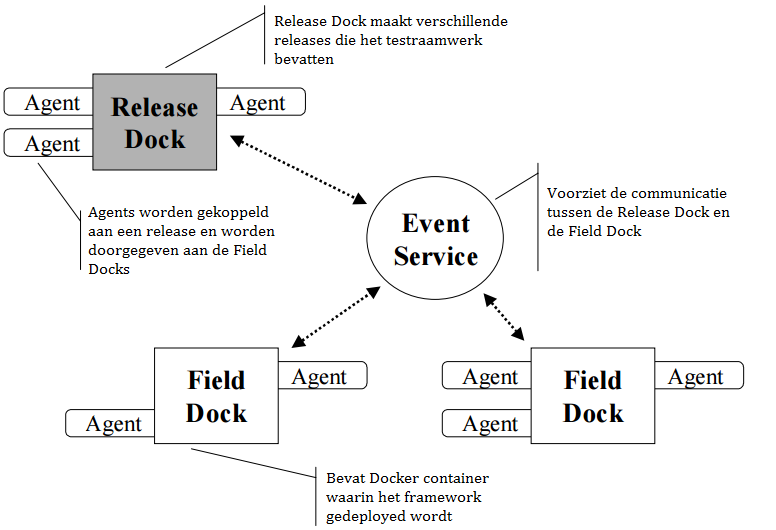
\includegraphics[scale=0.5]{afbeelding/softwareDockAangepast.png}}
\caption{Software Dock Architectuur \citep{hall1999cooperative}}
\label{fig:softwareDockAangepast}
\end{figure}

\paragraph{Release Dock}
Het release dock bevindt zich aan de serverzijde en bevat de code voor zowel de packager als de monitor van de clients.
Met hulp van de packager worden de verschillende installers geproduceerd.
Naast het produceren van installers zal het release dock instaan voor het monitoren van de field docks.
Hier wordt vooral gebruik gemaakt van de verschillende resultaten van de test die uitgevoerd worden tijdens het installatieproces.
Op de manier wordt achterhaalt welke installer geïnstalleerd werd op een field dock en welke fouten eventueel optraden tijdens het installatieproces.

\paragraph{Event Service}
%%% TODO
Nevens de verschillende docks beschrijft de software dock architectuur een Event Service.
Deze staat in voor het afhandelen van de communicatie tussen de verschillende docks.
Om dit te implementeren, wordt er beroep gedaan op Sectie~\vref{sec:event}.
Er worden evenwel enkele kleine aanpassingen gemaakt.
%%% TODO schrijven over lijsten die worden bijgehouden
De broker worden verschillende lijsten bijgehouden voor ieder type van bericht dat mogelijk is.
Bij het toekomen van een subscribe/unsubscribe bericht, zal de broker de nodige lijsten aanpassen zodat de zender van het bericht wordt toegevoegd of verwijderd.
Berichten in het netwerk zullen bestaan uit een set van attributen en waarden in een JSON formaat.
Het uiterlijk van zo'n bericht is gelijkaardig als het uiterlijk van een bericht in Figuur~\vref{fig:pubsubNot}.
In Listing~\vref{list:bericht} wordt een voorbeeld van een bericht weergegeven.
Ieder bericht heeft dezelfde set aan attributen die elk een eigen functie hebben:
\begin{itemize}
\item \emph{Timestamp}: ieder bericht zal op het moment van de creatie een timestamp krijgen.
De timestamp wordt uitgedrukt in seconden sinds epoch.
Op deze wijze wordt eenzelfde referentie punt gebruikt en is het mogelijk om de creatie van berichten in de tijd te ordenen.
\item \emph{Type}: ieder bericht hoort toe aan een bepaald type.
De verschillende types van berichten zijn: subscribe, unsubscribe, new, change, rapport, update, release.
Afhankelijk van het type bericht dat toekomt, bij zowel de broker als een dock, zal een andere actie ondernomen worden.
De eerste twee types zijn uitsluitend bedoelt voor de broker.
De volgende drie voor een release dock en de laatste twee voor de field docks.
\item \emph{ID}: naast een timestamp wordt aan ieder bericht een id meegegeven. 
Dit attribuut wordt meegegeven zodanig dat de field docks kunnen achterhalen of zij achterlopen op berichten.
\item \emph{Data}: Dit is het meest flexibele attribuut. 
Hier wordt de data meegegeven die hoort bij het bericht.
Als het type van een bericht ``subscribe'' is, dan zit in het data veld een lijst met alle types waarvoor de gebruiker zich voor wilt inschrijven.
\item \emph{Sender}: Het laatste attribuut dat wordt meegegeven is de zender van het bericht.
De broker moet bij een subscribe bericht kunnen achterhalen wie de zender is.
Op die manier weet de broker wie moet worden toegevoegd aan de nodige lijsten.
\end{itemize}

\begin{minipage}{\linewidth}
\begin{center}
\begin{lstlisting}[caption={Format voor een bericht},label={list:bericht}, xleftmargin=.3\textwidth]
{
 'timestamp': 1491982212.555,
 'type': 'subscribe',
 'id': 0,
 'data': {
   'type': [
     'new',
     'change',
     'rapport'
   ]
 },
 'sender': 'localhost'
}
\end{lstlisting}
\end{center}
\end{minipage}

\paragraph{Agenten}
%%schrijven over hoe de agenten werken en hoe ze gaan werken volgens de handelingen van ORYA
Naast de docks beschrijft de software dock architectuur ook agenten.
Deze staan in voor het uitvoeren van allerlei deployment gerelateerde handelingen.
Iedere agent is gekoppeld aan één stap uit de software levenscyclus die besproken werd in Sectie~\vref{sec:softwareLevenscyclus}.
Hiernaast zal aan iedere installer afkomstig van het release dock een subset van alle agenten toegevoegd en verscheept worden naar het field dock.
Op deze manier is het mogelijk om iedere stap in de levenscyclus van de installer te personaliseren.
Ieder agent zal een bepaalde set van handelingen uitvoeren die overeenkomt met een deployment proces die besproken werd in de ORYA case studie in Sectie~\vref{sec:ORYA}.
Net zoals bij ORYA wordt ieder deployment proces beschreven aan de hand van andere deployment processen en basis activiteiten.
Een voorbeeld:
Tijdens de creatie van een installer wordt een agent voorzien die instaat voor het installatieproces.
De agent wordt samen met de installer verscheept naar het field dock waarna de agent op het gepaste moment in actie schiet.
De agent begint met het hernoemen van de oude Docker container met daarin de vorige versie van een installer.
Hierna wordt een nieuwe container aangemaakt waarin de nieuwe installer wordt losgelaten.
Vervolgens zal de agent de installatie aanvangen en zullen de scripts horende bij de pakketten uitgevoerd worden in de container.
Zoals reeds werd aangegeven, zijn de handelingen van een agent gebaseerd op het model van ORYA.
Zo wordt het creëren van een nieuwe container in de installatie agent wordt gezien als zo'n basis activiteit.
In Bijlage~\vref{sec:flowcharts} zijn verschillende flowcharts terug te vinden die horen bij enkele types van agenten.
Door agenten te gebruiken, een strategie die ook gezien werd in de Atlas case studie in Sectie~\vref{sec:ATLAS}, wordt het mogelijk om alle stappen in de software levenscyclus uniek te behandelen.
Hiernaast kan bij iedere installer een andere set van agenten geassocieerd worden waardoor iedere installer verder gepersonaliseerd kan worden.

\subsection{Deployment environment}
De deployment environment komt overeen met de field dock in de software dock architectuur.
In de omgeving gaat de installer, afkomstig van de packager, uitgevoerd worden zodanig dat het test framework geïnstalleerd wordt.
Aan dit proces zijn de verschillende problemen verbonden die besproken werden in Sectie~\vref{sec:softwareLevenscyclus}.
Om de verschillende deployment problemen te vermijden en om ervoor te zorgen dat geen uitgebreide rollback strategieën nodig zijn, wordt een geïsoleerde omgeving voorzien waarin de software geïnstalleerd wordt. 
Dit wordt gerealiseerd aan de hand van virtualisatie technieken, meer bepaald aan de hand van Docker.
Docker wordt verkozen boven een gewone virtuele machine omdat het uitvoeren van handelingen (zoals opstarten, stoppen, \ldots) op een container minder resources en tijd vraagt in vergelijking met een virtuele machine.
Doordat een virtualisatie techniek wordt gebruikt, wordt het zeer eenvoudig om problemen tijdens de verschillende processen op te vangen.
In Figuur~\vref{fig:flow:install} en Figuur~\vref{fig:flow:rollback} is het duidelijk dat, door het gebruik van Docker, het rollback proces zeer eenvoudig is.
Figuur~\vref{fig:fieldDock} geeft weer op welke manier de agenten met de containers gaan communiceren en geeft ook weer hoe Docker wordt geïntegreerd in het geheel.

\begin{figure}[!ht]
\centering
\makebox[0pt]{\includegraphics[scale=0.5]{afbeelding/fieldDock.png}}
\caption{Structuur van een field dock}
\label{fig:fieldDock}
\end{figure}

De volledige architectuur wordt weergegeven in Figuur~\vref{fig:architectuur}.
In de figuur worden de verschillende docks afgebeeld samen met zowel Docker als de packager.
Met deze architectuur is het mogelijk om aan de slag te gaan en een goede oplossing te vinden voor het probleem van Televic.

\begin{figure}[!ht]
\centering
\makebox[0pt]{\includegraphics[scale=0.5]{afbeelding/architectuur.png}}
\caption{Architectuur van het prototype}
\label{fig:architectuur}
\end{figure}
